\section{Flujo de trabajo}
\label{ch:propuesta:sec:flujoDeTrabajo}

Actualmente existen flujos de trabajo para la extracción de supeficies \cite{Ruprecht94ascheme}\cite{Dietrich_marchingcubes}, los cuales intentan generar superficies sin los principales problemas topológicos explicados en \ref{subsec:marchingCubes:consecuencias}. El flujo de trabajo propuesto en esta investigación se muestra en la fugura \ref{f:flujoDeTrabajo:flujoDeTrabajo}

\begin{figure}[htb]
\centering
	\includegraphics[width=0.5\textwidth]{images/misc/workflow.pdf}
\caption{Flujo de trabajo propuesto}
\label{f:flujoDeTrabajo:flujoDeTrabajo}
\end{figure}

Cada uno de estos pasos serán explicados a continuación.
\newpage

\subsection{Extracción de datos}
\label{ch:propuesta:sec:extraccionDeDatos}

En primera instancia, para extraer una superficie desde una nube de puntos, es necesario recolectar estos puntos, para eso existen diversas técnicas y propósitos. Para el propósito de esta investigación, el formato de los datos debe ser un \emph{dataset} de imágenes coaxiales que individualmente muestran una seccion planar de la superficie que se quiere extraer, y en conjunto describen la superficie completa.

\subsubsection{Imágenes por resonancia magnética}
\label{ch:propuesta:sec:extraccionDeDatos:subsec:imagenesPorResonanciaMagnetica}

En el análisis de imágenes médicas, en ocaciones se necesita visualizar \emph{datasets} volumétricos, cortes en tres dimensiones de los órganos que se quieren estudiar, como las imágenes obtenidas por resonancia magnética (\emph{MRI}, de sus siglas en inglés \emph{Magnetic resonance imaging}).

Las imágenes por resonancia magnética son una técnica de imagenología usada principalmente en el área médica para producir imágenes de alta calidad del interior del cuerpo humano. Estas imágenes son basadas en el principio de la resonancia nuclear magnética, una técnica espectroscópica usada por científicos para obtener información física y química acerca de las moléculas. Ya en el año 2003 existían aproximadamente mas de diez mil unidades de resonancia magnética y aproximadamente setenta y cinco millones de exámenes realizados por año \footnote{Joseph P. Hornak, Ph.D. \textit{The Basics of MRI}, http://www.cis.rit.edu/htbooks/mri/ (19 sept. 2012).}

Las imágenes obtenidas de estos exámenes pueden ser pensadas como imágenes en tres dimensiones donde cada \emph{pixel} (o \emph{voxel}, elemento de volúmen) representa una cantidad medible de volumen en alguna posición $(x, y, z)$ del espacio. Un ejemplo de estas imágenes se muestra en la figura \ref{f:flujoDeTrabajo:mri_joe} \footnote{MRI, CPO Abdomen Total, paciente Joe Cabezas Campos, estudio 040501000, Integramedica, Av. Libertador Bernardo O'Higgins 1620, 26 junio 2012 19:35}

\begin{figure}[p]
\centering
	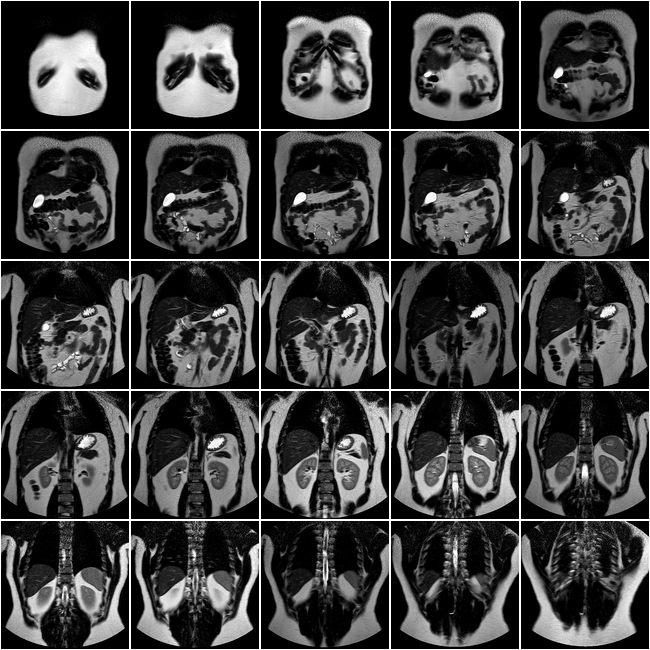
\includegraphics[width=1.0\textwidth]{images/misc/mri_joe.png}
\caption{Un \emph{dataset} de 28 imágenes de un examen de resonancia magnética}
\label{f:flujoDeTrabajo:mri_joe}
\end{figure}

Una forma de visualizar el cuerpo en tres dimensiones es extrayendo una \emph{isosuperficie} usando el algoritmo de \emph{Marching Cubes}.

En esta investigación, la totalidad de los dataset usados para la implementación del algoritmo de \emph{Marching Cubes} son extraidos de imágenes de resonancia magnética.
\newpage

\subsubsection{Funciones en tres dimensiones}
\label{ch:propuesta:sec:extraccionDeDatos:subsec:funcionesEnTresDimensiones}

Otra forma de obtener puntos en un espacio es usando una función matemática de tres dimensiones que asocie cualquier punto de un espacio a un valor escalar. El algoritmo de \emph{Marching Cubes} hace uso de una discretización del espacio ya que cada vértice de cada cubo está apoyado en un punto discreto del espacio, debido a la continuidad de una función de tres dimensiones, es posible escoger cualquier tamaño para los cubos, lo que hace posible escoger la resolución que se desee y con ello tener un malla en tres dimensiones mas detallada como se explica en \ref{subsec:marchingCubes:consecuencias}, pero necesariamente con más triángulos lo que puede no ser óptimo.

Si se desea extraer la superficie descrita por una función continua en tres dimensiones, para esta investigación es necesario generar las imágenes de las curvas de nivel que finalmente cumplirán la misma función que las imágenes por resonancia magnética. Un ejemplo de una función continua es la ecuacion \ref{ecuacionContinua}

\begin{equation}
f(x,y) = \frac{ \sin{(\sqrt{x^2+y^2})} }{ \sqrt{x^2+y^2} }
\label{ecuacionContinua}
\end{equation}

y sus respectivos gráficos y curvas de nivel se muestra en la figura \ref{c:flujo:greaficoDeLaEcuacion}

\begin{figure}[h]

	\begin{subfigure}[b]{0.45\textwidth}
		\centering
		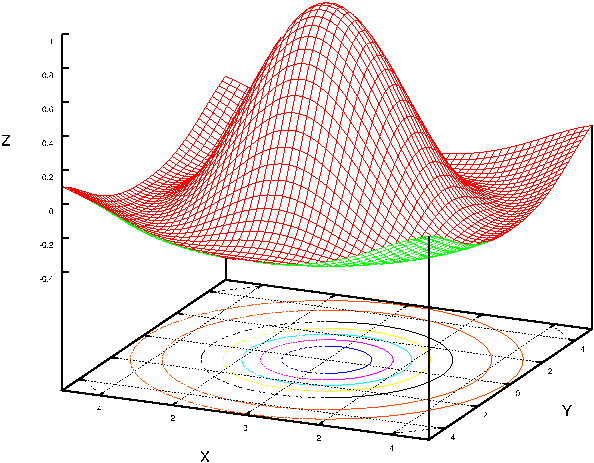
\includegraphics[width=\textwidth]{images/misc/contour_1_using_eps2eps.pdf}
		\caption{Superficie en tres dimensiones}
		\label{c:flujo:superficieEnTresDimensiones}
	\end{subfigure}
	~~
	\begin{subfigure}[b]{0.45\textwidth}
		\centering
		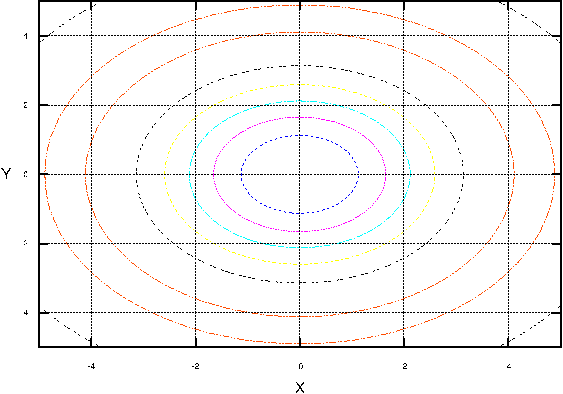
\includegraphics[width=\textwidth]{images/misc/contour_2_using_eps2eps.pdf}
		\caption{Gráfico de curvas de nivel}
		\label{c:flujo:graficoDeCurvasDeNivel}
	\end{subfigure}

	\caption{Gráfico de la ecuación \ref{ecuacionContinua}}
	\label{c:flujo:greaficoDeLaEcuacion}

\end{figure}

Finalmente, cada una de las lineas de las curvas de nivel mostradas en \ref{c:flujo:graficoDeCurvasDeNivel}, representa una imagen de entrada para el algoritmo.

\subsection{Conversión de imágenes}
\label{ch:propuesta:sec:conversionDeImagenes}

Como se plantea en la sección anterior (\ref{ch:propuesta:sec:extraccionDeDatos}), existen varias formas de extraer los datos, por lo que, dependiendo la técnica usada es posible que las imágenes de entrada vengan en diversos formatos tambien como se explicará mas adelante en \ref{ch:implementacion:sec:datosDeEntrada:subsec:formatodelasimagenesdeentrada}.

Es por esto que para garantizar una independencia de la implementacion hecha en esta investigación con el formato de las imágenes de entrada que se necesita un paso que unifique las diversas formas de extracción de datos para que puedan ser usadas en esta implementación, los detalles de la implementacion de esto se verá en el capitulo \ref{ch:implementacion}.

Una vez que se asegure que las imágenes de entrada usan el mismo formato, la implementación puede utilizar esta información previa para trabajar haciendo uso de sólamente un formato en común, haciendo la implementación mas simple. El formato escogido es el formato PGM (\emph{Portable GreyMap}), detalles de su utilización se verán en la sección \ref{ch:implementacion:sec:formatounicoescogido}.

\subsection{Selección del isovalor}
\label{ch:propuesta:sec:seleccionDelIsovalor}

Una vez que se tienen las imágenes de entradas, es momento de escoger una constante que definirá aquellos \emph{pixeles} que estarán dentro o fuera de la superficie que se desea extraer en cada imágen, por lo tanto, la superficie está determinada por este valor llamado \jcq{isovalor}.

Este paso no es trivial, ya que requiere retroalimentación de la superficie extraída, pues en el caso de las imágenes médicas de resonancia magnética, la elección del isovalor puede marcar la diferencia entre ver un cuerpo al nivel del cráneo o al nivel de los huesos internos de éste como se muestra en la figura \ref{c:flujo:superficieDeUnaCalaveraADistintosNivelesDeIsovalor} donde se observa que al aumentar el valor porcentual del isovalor cada vez hay menos puntos en el espacio que sean menores al isovalor, por lo que cada vez la superficie es distinta. La correcta elección del isovalor en las imágenes determina finalmente el nivel de la superficie que se quiere extraer, por ejemplo, si se escoge un valor cero, significa que todas los pixeles quedarán fuera y por lo tanto ningún cubo en el proceso de extracción de superficie tendrá algún vértice marcado como interno, luego, no se generará ningún triángulo y se creará una superficie nula, lo mismo ocurre si se escoge un isovalor que sea igual al máximo valor posible en las imágenes.


\begin{figure}[h]

	\begin{subfigure}[b]{0.30\textwidth}
		\centering
		\fbox{
			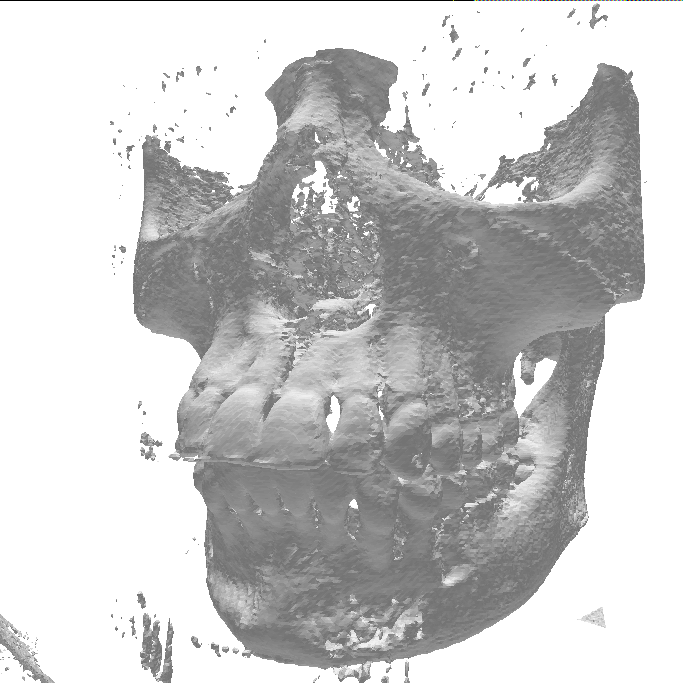
\includegraphics[width=\textwidth]{images/flujo/isovalue/screenshot_15.png}
		}
		\caption{Isovalor de 15\%}
	\end{subfigure}
	\quad
	\begin{subfigure}[b]{0.30\textwidth}
		\centering
		\fbox{
			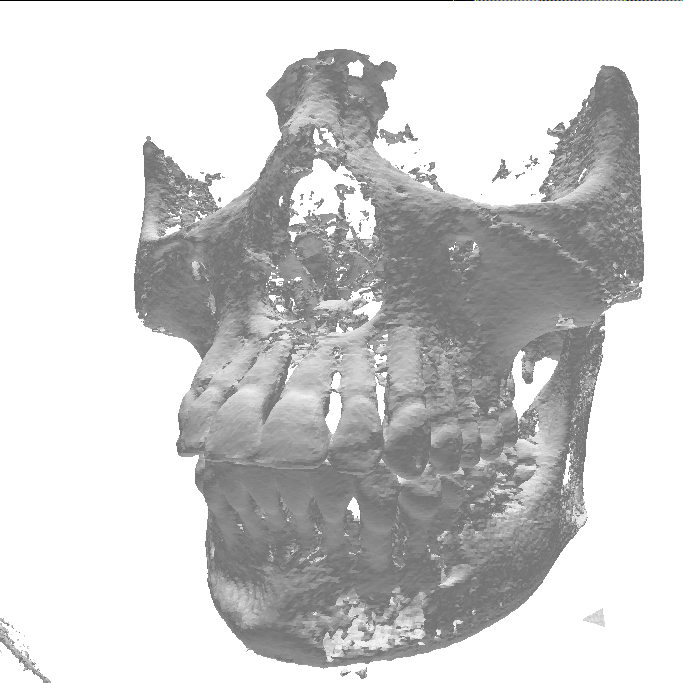
\includegraphics[width=\textwidth]{images/flujo/isovalue/screenshot_20.png}
		}
		\caption{Isovalor de 20\%}
	\end{subfigure}
	\quad
	\begin{subfigure}[b]{0.30\textwidth}
		\centering
		\fbox{
			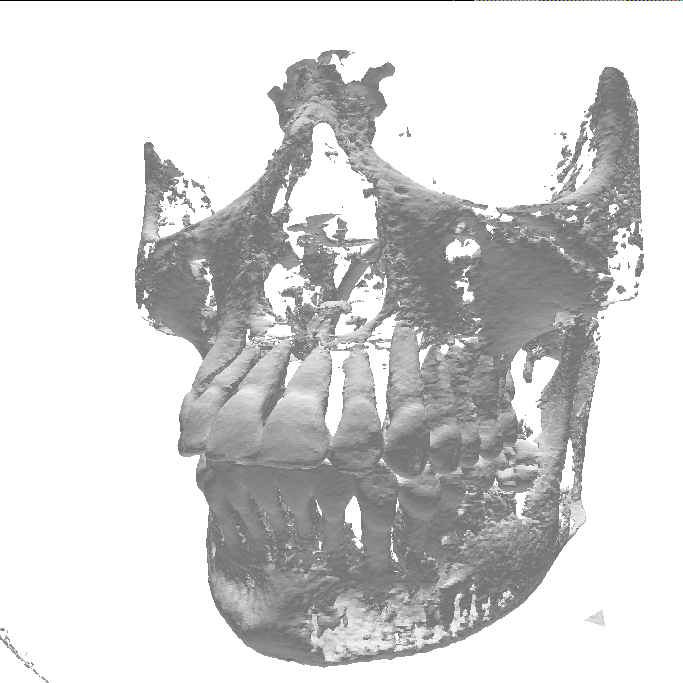
\includegraphics[width=\textwidth]{images/flujo/isovalue/screenshot_25.png}
		}
		\caption{Isovalor de 25\%}
	\end{subfigure}


	\begin{subfigure}[b]{0.30\textwidth}
		\centering
		\fbox{
			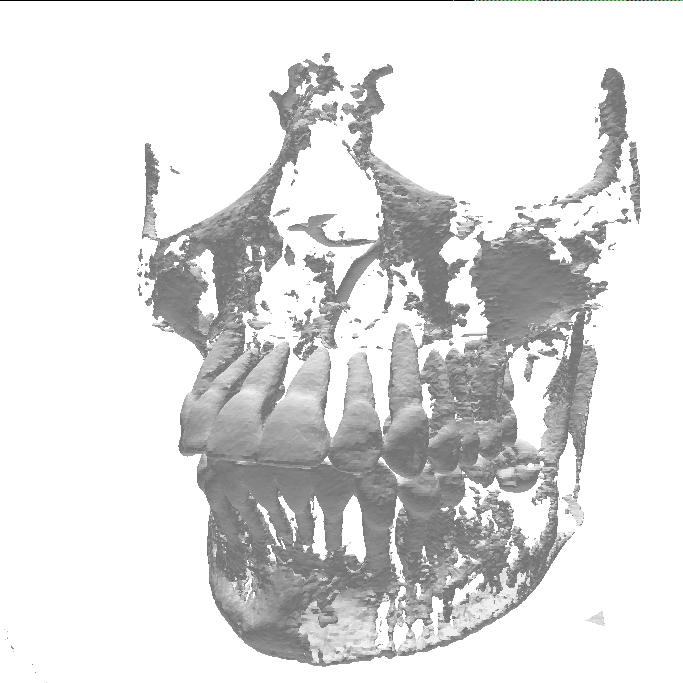
\includegraphics[width=\textwidth]{images/flujo/isovalue/screenshot_30.png}
		}
		\caption{Isovalor de 30\%}
	\end{subfigure}
	\quad
	\begin{subfigure}[b]{0.30\textwidth}
		\centering
		\fbox{
			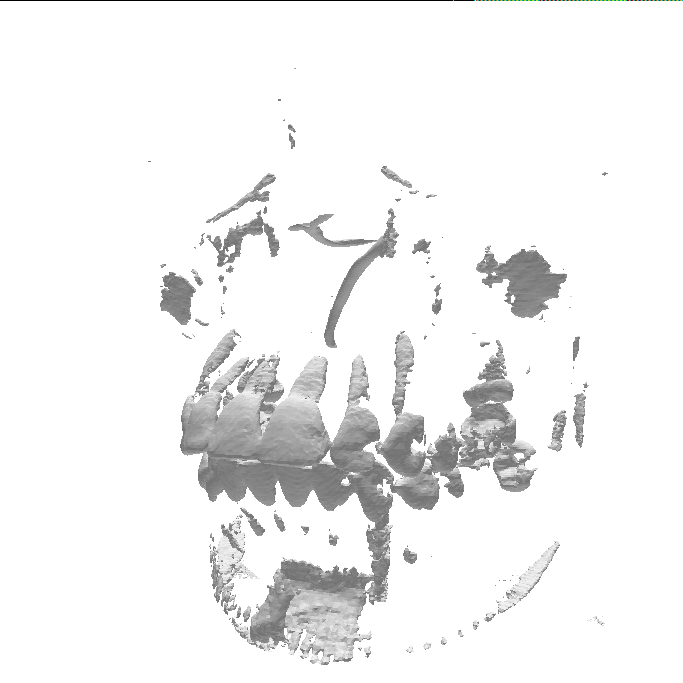
\includegraphics[width=\textwidth]{images/flujo/isovalue/screenshot_40.png}
		}
		\caption{Isovalor de 40\%}
	\end{subfigure}
	\quad
	\begin{subfigure}[b]{0.30\textwidth}
		\centering
		\fbox{
			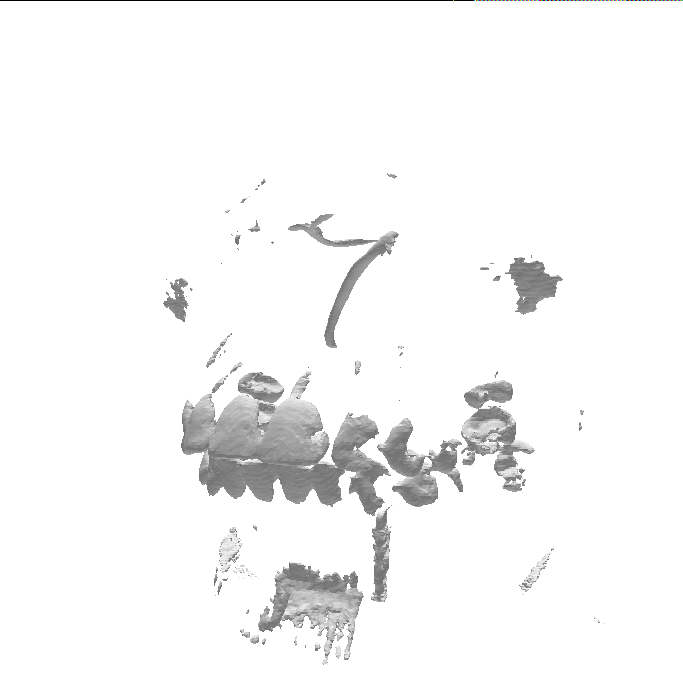
\includegraphics[width=\textwidth]{images/flujo/isovalue/screenshot_45.png}
		}
		\caption{Isovalor de 45\%}
	\end{subfigure}


	% \begin{subfigure}[b]{0.30\textwidth}
	% 	\centering
	% 	\fbox{
	% 		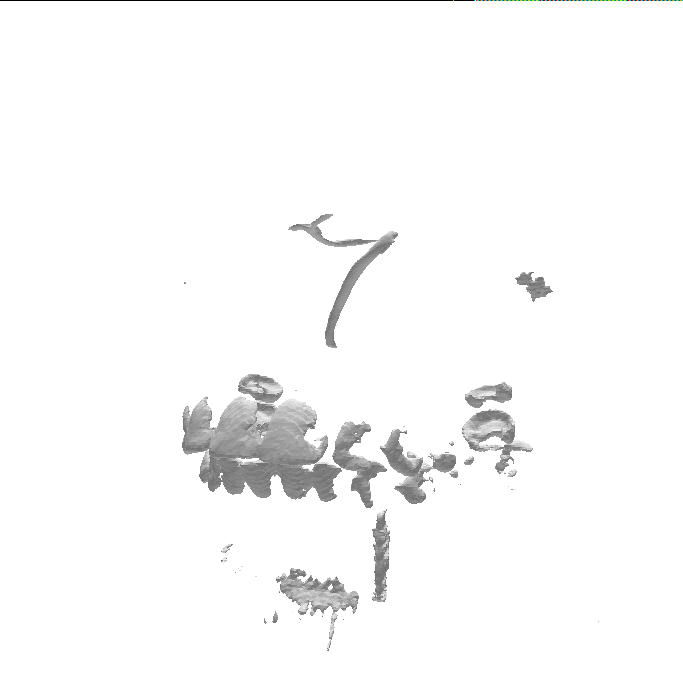
\includegraphics[width=\textwidth]{images/flujo/isovalue/screenshot_50.png}
	% 	}
	% 	\caption{Isovalor de 50\%}
	% \end{subfigure}
	% \quad
	% \begin{subfigure}[b]{0.30\textwidth}
	% 	\centering
	% 	\fbox{
	% 		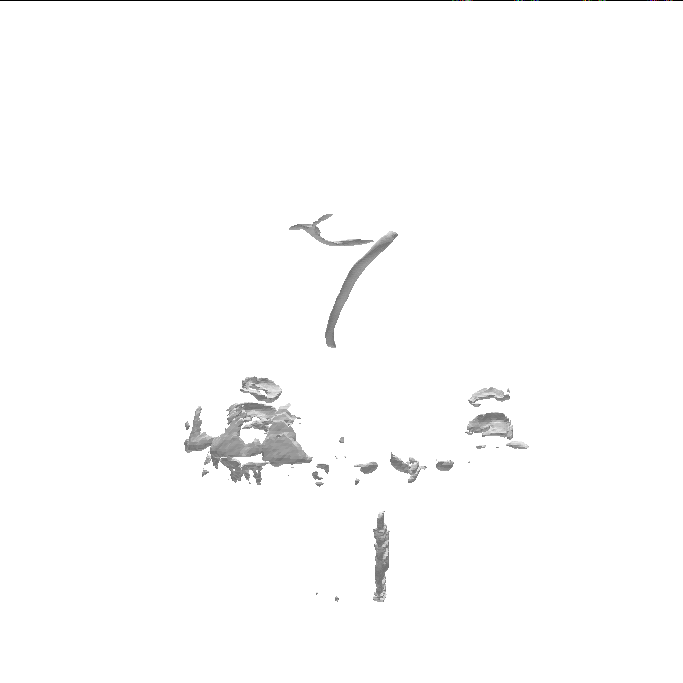
\includegraphics[width=\textwidth]{images/flujo/isovalue/screenshot_60.png}
	% 	}
	% 	\caption{Isovalor de 60\%}
	% \end{subfigure}
	% \quad
	% \begin{subfigure}[b]{0.30\textwidth}
	% 	\centering
	% 	\fbox{
	% 		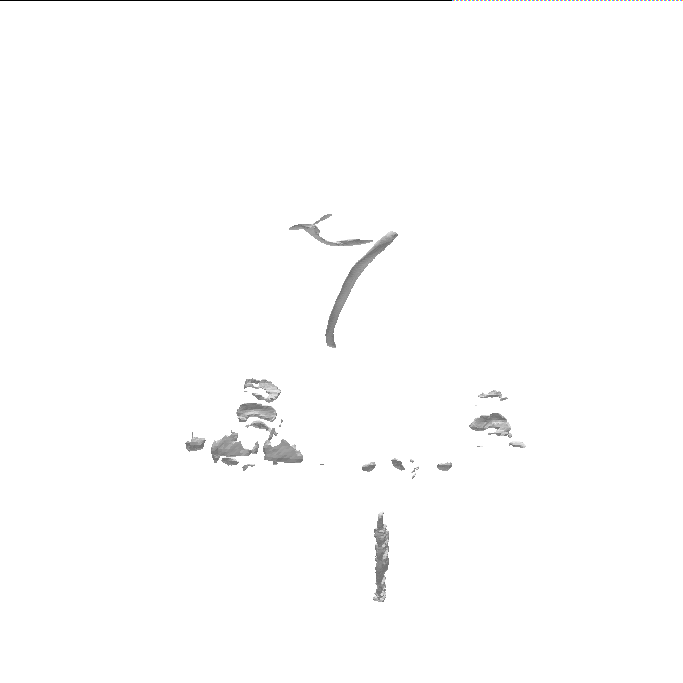
\includegraphics[width=\textwidth]{images/flujo/isovalue/screenshot_65.png}
	% 	}
	% 	\caption{Isovalor de 65\%}
	% \end{subfigure}

	\caption{Superficie de una calavera a distintos niveles de isovalor}
	\label{c:flujo:superficieDeUnaCalaveraADistintosNivelesDeIsovalor}

\end{figure}

En esta implementación, con el fin de garantizar una independencia de las imágenes de entrada con la manipulación del iso valor, es que el valor del isovalor se escoge porcentualmente, es decir, $0\%$ siginifica que el isovalor vale cero, y una elección de $100\%$ significa que el isovalor vale el máximo valor posible. Esto es porque dependiendo del nivel de profundidad de color de las imágenes, estas pueden ser expresadas entre 0--255 valores (8 bits) y 0--65536 valores (16 bits).

\subsection{Extracción de la superficie}
\label{ch:propuesta:sec:extraccionDeLaSuperficie}

Luego de escoger el isovalor adecuado, el siguiente paso es extraer la superficie usando el isovalor, por esto se le llama \jcq{isosuperficie}.

Esta investigación tiene su mayor enfoque en este punto ya que es en este paso donde se utiliza el algoritmo de \emph{Marching Cubes} para la extracción. Se desarrolló un \emph{software} que genera la superficie usando un isovalor porcentual ajustable por el usuario, y permite visualizar y navegar en tres dimensiones el modelo generado, una imagen del programa desarrollado se muestra en la figura \ref{f:flujoDeTrabajo:visualizer_1}. La principal característica de este visualizador es que es posible editar el isovalor y ver el cambio de la isosuperficie en tiempo real, permitiendo de esta manera corregir el isovalor usado para obtener el nivel de isovalor apropiado.

\begin{figure}[h]
\centering
	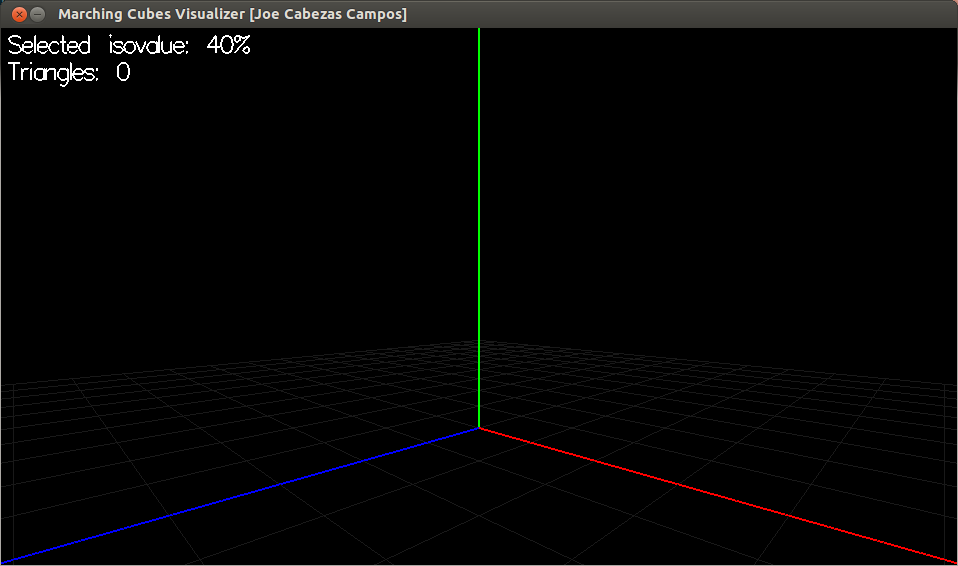
\includegraphics[width=1.0\textwidth]{images/visualizer/visualizer_1.png}
\caption{Programa visualizador de superficies generadas usando \emph{Marching Cubes}}
\label{f:flujoDeTrabajo:visualizer_1}
\end{figure}

\subsubsection{Interfaz}
\label{ch:propuesta:sec:extraccionDeLaSuperficie:subsec:interfaz}

La interfaz es simple, el programa muestra en su completitud una ventana OpenGL\footnote{http://www.opengl.org/} y en la esquina superior izquierda un panel de estado que indica el isovalor actual (porcentual) y la cantidad de triángulos de la superficie, como se muestra en la figura \ref{f:flujoDeTrabajo:interface}

\begin{figure}[h]
\centering
	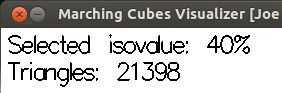
\includegraphics[width=0.5\textwidth]{images/visualizer/interface.png}
\caption{Panel de estado, con un isovalor del 40\%, se crea una superficie que esta formada por $172416$ triángulos.}
\label{f:flujoDeTrabajo:interface}
\end{figure}

\subsubsection{Modo de uso}
\label{ch:propuesta:sec:extraccionDeLaSuperficie:subsec:modoDeUso}

Es posible usar el programa tanto con teclado como con un control de Xbox360\textsuperscript{\textregistered}\footnote{http://www.microsoft.com/hardware/en-us/p/xbox-360-controller-for-windows (20 sept. 2012)}.

El programa además puede capturar imágenes en formato \emph{PNG} (Portable Network \mbox{Graphics}\footnote{http://www.libpng.org/pub/png/}), generando imágenes con nombre cuyo formato es:

\begin{quote}
	screenshot\_\textbf{\textless isovalor porcentual\textgreater}.png
\end{quote}

También es posible exportar la superficie que se esta visualuzando a un archivo de modelo 3D (archivo \emph{OFF}), para así poder ser importado en otro programa que acepte este formato como geomview\footnote{http://www.geomview.org/}, como se muestra en la figura \ref{f:flujoDeTrabajo:geomview}

\begin{figure}[!htb]
\centering
	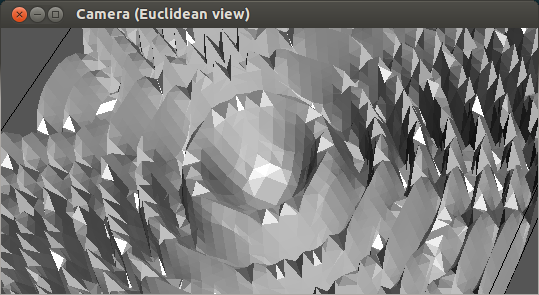
\includegraphics[width=0.7\textwidth]{images/visualizer/geomview.png}
\caption{Superficie generada en el visualizador, importada como archivo OFF en \mbox{geomview}}
\label{f:flujoDeTrabajo:geomview}
\end{figure}

\newpage
A continuación se muestra una tabla con las teclas de control\footnote{Imágenes obtenidas desde https://github.com/sgraham/gamepad.js/ (20 sept. 2012)}\footnote{Xbox 360 Icon Pack por Jeff Jenkins, @sinnix, http://sinnix.net/downloads/?did=1 (20 sept. 2012)}:

\begin{longtable}[c]{
	|>{\centering}m{3.0cm}<{\centering}|
	m{3cm}||
	l|
}
\hline
Teclado & Control Xbox360 & Acción \\ \hline
	\huge{\keystroke{\large{W}}} &
	
\includegraphics[scale=0.4]{images/visualizer/xbox360/leftStick.png} (arriba) &
	Avanzar
	\\ \hline

	\huge{\keystroke{\large{A}}} &
	
\includegraphics[scale=0.4]{images/visualizer/xbox360/leftStick.png} (izquierda) &
	Desplazarse hacia la izquierda
	\\ \hline

	\huge{\keystroke{\large{S}}} &
	
\includegraphics[scale=0.4]{images/visualizer/xbox360/leftStick.png} (derecha) &
	Retroceder
	\\ \hline

	\huge{\keystroke{\large{D}}} &
	
\includegraphics[scale=0.4]{images/visualizer/xbox360/leftStick.png} (abajo) &
	Desplazarse hacia la derecha
	\\ \hline

	\huge{\keystroke{\large{$\downarrow$}}} &
	\centering 
\includegraphics[scale=0.4]{images/visualizer/xbox360/leftShoulder1.png} &
	Descender
	\\ \hline

	\huge{\keystroke{\large{$\uparrow$}}} &
	\centering 
\includegraphics[scale=0.4]{images/visualizer/xbox360/rightShoulder1.png} &
	Ascender
	\\ \hline

	\huge{\keystroke{\large{$\leftarrow$}}} &
	
\includegraphics[scale=0.4]{images/visualizer/xbox360/rightStick.png} (izquierda) &
	Girar hacia la izquierda
	\\ \hline

	\huge{\keystroke{\large{$\rightarrow$}}} &
	
\includegraphics[scale=0.4]{images/visualizer/xbox360/rightStick.png} (derecha) &
	Girar hacia la derecha
	\\ \hline

	\huge{\keystroke{\large{F1}}} \normalsize{ó} \huge{\keystroke{\large{-}}} &
	\centering 
\includegraphics[scale=0.6]{images/visualizer/xbox360/leftShoulder0.png} &
	Disminuir el isovalor
	\\ \hline

	\huge{\keystroke{\large{F2}}} \normalsize{ó} \huge{\keystroke{\large{+}}} &
	\centering 
\includegraphics[scale=0.6]{images/visualizer/xbox360/rightShoulder0.png} &
	Aumentar el isovalor
	\\ \hline

	\huge{\keystroke{\large{Enter}}} &
	\centering 
\includegraphics[scale=0.6]{images/visualizer/xbox360/start.png} &
	Generar isosuperficie (\emph{Marching Cubes})
	\\ \hline

	\huge{\keystroke{\large{Backspace}}} &
	\centering 
\includegraphics[scale=0.6]{images/visualizer/xbox360/select.png} &
	Destruye isosuperficie
	\\ \hline

	\huge{\keystroke{\large{R}}} &
	\centering 
\includegraphics[scale=0.6]{images/visualizer/xbox360/dpadLeft.png} &
	Rotar superficie en eje X (horario)
	\\ \hline

	\huge{\keystroke{\large{F}}} &
	\centering 
\includegraphics[scale=0.6]{images/visualizer/xbox360/dpadRight.png} &
	Rotar superficie en eje X (antihorario)
	\\ \hline

	\huge{\keystroke{\large{T}}} &
	\centering 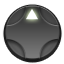
\includegraphics[scale=0.6]{images/visualizer/xbox360/dpadUp.png} &
	Rotar superficie en eje Y (horario)
	\\ \hline

	\huge{\keystroke{\large{G}}} &
	\centering 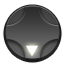
\includegraphics[scale=0.6]{images/visualizer/xbox360/dpadDown.png} &
	Rotar superficie en eje Y (antihorario)
	\\ \hline

	\huge{\keystroke{\large{P}}} &
	\centering 
\includegraphics[scale=0.6]{images/visualizer/xbox360/faceButton0.png} &
	Capturar imagen (\emph{screenshot})
	\\ \hline

	\huge{\keystroke{\large{O}}} &
	\centering 
\includegraphics[scale=0.6]{images/visualizer/xbox360/faceButton1.png} &
	Exportar modelo 3D (archivo \emph{OFF})
	\\ \hline

	\huge{\keystroke{\large{F11}}} &
	\centering 
\includegraphics[scale=0.6]{images/visualizer/xbox360/faceButton2.png} &
	Alternar modo pantalla completa
	\\ \hline

	\huge{\keystroke{\large{Esc}}} &
	\centering 
\includegraphics[scale=0.6]{images/visualizer/xbox360/faceButton3.png} &
	Salir
	\\ \hline

\end{longtable}

% \subsection{Refinamiento}
% \label{ch:propuesta:sec:refinamiento}